%% This is file `elsarticle-template-1-num.tex',
%% Copyright 2009 Elsevier Ltd
% \documentclass[final,5p,times,twocolumn]{elsarticle}
\documentclass[final,3p,times]{elsarticle}


\usepackage{graphicx}
\usepackage{amsmath, amssymb}
\usepackage{epstopdf}
\usepackage{lmodern}
\usepackage[latin9]{inputenc}
\usepackage[T1]{fontenc}
\usepackage{color}
\usepackage{float}
\usepackage{tabularx,ragged2e,booktabs,caption}
\usepackage{breqn}
\usepackage{pgfplots}
\pgfplotsset{compat=1.5}
\usepackage{subcaption}

\newcommand{\mbf}{\mathbf}

%% Figure placeholder: keeps captions/labels intact while artwork is pending.
\newcommand{\figplaceholder}[1]{%
  \fbox{\parbox[c][3.2cm][c]{0.85\linewidth}{\centering%
    \textbf{[FIGURE PLACEHOLDER]}\\[4pt]\texttt{#1}}}}

\bibliographystyle{elsarticle-harv}\biboptions{authoryear}

\journal{International Journal of Solids and Structures}

\begin{document}

\begin{frontmatter}

\title{Surface and Interfacial Tension Effects on the Wrinkling of Multilayer Dielectric Elastomer Films}

\author[ss]{Saman Seifi}
\ead[ss]{samansei@bu.edu}
\address[ss]{Department of Mechanical Engineering, Boston University, Boston, MA 02215}
\author[hsp]{Harold S. Park}
\ead[hsp]{parkhs@bu.edu}
\address[hsp]{Department of Mechanical Engineering, Boston University, Boston, MA 02215}

\begin{abstract}
Multilayer dielectric-elastomer films---a stiff dielectric skin bonded to a softer compliant substrate, or laminates of several dissimilar layers---are increasingly used in soft actuators and sensors, and when operated in fluidic environments they experience surface tension not only on their outer surface but also, through the mismatch of interfacial energies, on the buried interfaces between layers. Here we extend the elastocapillary wrinkling analysis of compressed dielectric elastomers to multilayer laminates. Building on the single-layer Young--Laplace framework, we formulate the bifurcation problem for a bonded bilayer carrying a free-surface tension and an independent interfacial tension, and generalize it to an arbitrary $N$-layer stack. Interfacial surface energy enters as a Laplace-pressure jump in the normal traction across the interface, raising the critical strain and coarsening the selected wavelength much as free-surface tension does. For laminates of three or more layers a qualitatively new effect emerges: a sufficiently large free-surface tension flattens the outer surface while a buried stiff layer continues to buckle, so that surface tension selects which interface fails first. The predictions are verified with nonlinear finite-element simulations in which the same edge-based Young--Laplace surface stress is applied on internal interfaces as on free surfaces.
\end{abstract}

\begin{keyword}
Wrinkling Instability \sep Elastocapillary \sep Interfacial Energy \sep Multilayer Films \sep Perturbation Analysis
\end{keyword}

\end{frontmatter}

\section{Introduction}

Because soft materials like gels and elastomers often operate under states of compression, there have been significant efforts to examine their mechanical stability under such loading~\citep{Biot1963,gent1999surface,biot1965mechanics,tanaka1987mechanical,gent2005elastic,hong2009formation}. Recently, efforts have focused on examining the stability of surfaces due to the formation of instabilities such as wrinkles and creases under compression~\citep{cao2012wrinkling,li2012mechanics,jin2014creases,cai2012creasing,hong2013crease,weiss2013creases}. The studies of wrinkling instabilities have typically been analytical in nature, based on linear perturbation analysis, which enables predictions of critical strains and instability wavelengths in these soft structures. These studies have also been insightfully combined with experiments~\citep{cai2010osmotic,cai2012creasing,Jin2015a}, and also numerical (finite element) analyses~\citep{cao2012wrinkling,jin2015smoothening,Jin2015a,wangJAM2014,wangMRS2016}.  

More recently, linear perturbation analyses have been applied to an interesting class of soft, active materials - dielectric elastomers (DEs). These materials have drawn significant interest due to the large deformations they can undergo resulting from applied electrostatic loading~\citep{carpiSCIENCE2010,brochuMRC2010,biddissMEP2008,mirMT2007}. Furthermore, DEs often form surface instabilities like creasing, wrinkling and cratering, which have been studied via experiment, theory and computation~\citep{suoAMSS2010,planteIJSS2006,zhouIJSS2008,wangAM2012,shivapoojaAM2013,wangPRL2011a,parkIJSS2012,parkCMAME2013}, and also using analytic techniques based on stability analyses~\citep{zhaoAPL2007,zhao2009electromechanical} and the nonlinear field theory of~\citet{suoJMPS2008}.

While DEs have drawn significant interest in recent years, many promising technological innovations, such as generating electromechanical motion during magnetic resonance imaging~\citep{Carpi2008mri}, operating soft, underwater robots~\citep{rusNATURE2015,kimTB2013}, manipulating microfluidic flow~\citep{Holmes2013}, focusing a tunable lens~\citep{Carpi2011}, the preparation of bioinspired surfaces~\citep{shivapoojaAM2013}, underwater grippers~\citep{Laschi2012} and soft body locomotion~\citep{Marchese2014}, involve operation of the DE in fluidic environments, where elastocapillary effects due to surface tension can become prominent~\citep{romanJPCM2010,liuAMS2012}. While prior works have examined either the effects of surface tension alone on surface instabilities in elastomers~\citep{chenPRL2012} and hydrogels~\citep{kangSM2010}, or the coupled effects of surface tension and electric fields on surface instabilities in constrained DE films~\citep{seifiIJSS2016,wangJMPS2016}, a general stability analysis of compressed DE films subject to both surface tension and electric fields has not been performed.  

The objective of this work is to extend the elastocapillary analysis of surface instabilities in DEs from a single layer to \emph{multilayer} laminates, in which surface energy acts both on the free outer surface and on the buried interfaces between dissimilar layers. Building on the single-layer Young--Laplace framework, we first summarize the perturbation analysis of a compressed single film, then formulate the bifurcation problem for a bonded bilayer with an independent interfacial tension, generalize it to an $N$-layer stack, and verify the predictions with nonlinear finite-element simulations in which the same Young--Laplace surface stress is applied on internal interfaces.

\section{Governing Equations and Incremental Forms}
\label{AppexA}

We first present, for a DE film subject to surface tension and under compressive loading, the governing equations and their incremental forms. We assume that the surface of the film is subject to Young-Laplace boundary conditions in order to account for elastocapillary effects on the surface~\citep{saksonoCM2006}. We restrict attention to mechanical (compressive) loading throughout; the electrostatic actuation of these films is treated in the companion single-layer study. The perturbation analysis we utilize is based on those performed by \citet{cai2010osmotic,kangSM2010,jin2014creases,Jin2015a}

\subsection{Dielectric Elastomer Subject to Surface Tension}

\begin{figure}
	\centering
	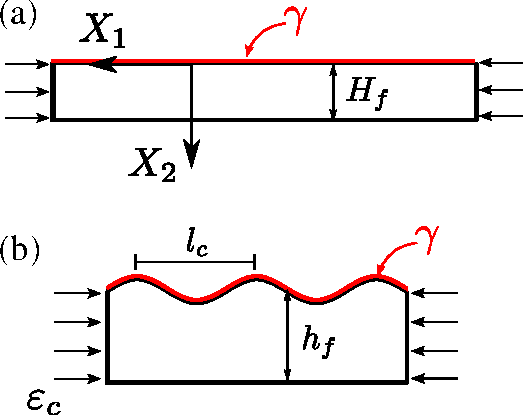
\includegraphics[width=0.78\linewidth]{pics/wrinkle_mech1.pdf}
	\caption{A perfectly flat film subject to compression and surface tension $\gamma$. (a) Undeformed configuration; (b) the formation of wrinkles with wavelength $l_c$. }
	\label{fig:mechfig}
\end{figure}

We first consider a DE film under compression, that is also subject to surface tension effects on its top surface, as illustrated in Figure (\ref{fig:mechfig}). The deformation of the body is described by the field $\mathbf{x}(\mathbf{X})$. The deformation gradient tensor $\mathbf{F}$ is defined as:
\begin{equation}
	\mathbf{F}=\nabla \mathbf{x}
	\label{eq:defgrad1}
\end{equation}
The DE is modeled as an incompressible neo-Hookean material with the free energy density function:
\begin{equation}
	W(\mathbf{F})=\frac{\mu}{2}\mathbf{F} : \mathbf{F}-\pi(\det{\mathbf{F}}-1)
	\label{eq:neoHookean}
\end{equation}
where $\mathbf{A} : \mathbf{B} = \text{tr}(\mathbf{A}^T \mathbf{B})$ denotes the tensor inner product. The first Piola-Kirchhoff (nominal) stress tensor $\mathbf{S}$ can be derived as:
\begin{equation}
	\mathbf{S}=\frac{\partial W(\mathbf{F})}{\partial \mathbf{F}}=\mu\mathbf{F}-\pi \mathbf{F}^{-T}
	\label{eq:mechstress1}
\end{equation}
where $\mu$ is the shear modulus, and $\pi=\pi(\mathbf{X})$ is the Lagrange multiplier to enforce the constraint of incompressibility: $J=\det{\mathbf{F}}=1$. 
The nominal stress satisfies the reference equilibrium equation:
\begin{equation}
	\nabla \cdot \mathbf{S} = \mathbf{0}
	\label{eq:equil_equ}
\end{equation}

On the surface of the body the film is subjected to the Young-Laplace boundary condition~\citep{saksonoCM2006} with surface tension $\gamma$:
\begin{equation}
	\mathbf{S}\mathbf{N}dA=2\gamma\kappa \mathbf{n} da
	\label{eq:YLBC}
\end{equation}
where $\mathbf{N}$ is the unit normal vector to the surface of the body in the undeformed state, $\mathbf{n}$ is the unit normal vector in the current state, and $\kappa$ is the mean curvature of the surface. 

We now add a perturbation into the state of finite deformation with position $\mathbf{x}_{0}(\mathbf{X})$, deformation gradient $\mathbf{F}_{0}(\mathbf{X})$ and nominal stress $\mathbf{S}_{0}(\mathbf{X})$. If the deformation in the $z$-direction is constrained, only 2D plane strain deformation is considered. The background deformation gradient of this state is
\begin{equation}
\mathbf{F}_{0}=
	\begin{bmatrix}
		\lambda & 0  \\
		0 & 1/\lambda \\
	\end{bmatrix}
\end{equation}
Therefore the corresponding base position is $\mathbf{x}_0 = \mathbf{F}_{0}\mathbf{X}$. Now by adding a small displacement perturbation $\delta\mathbf{x}$ and pressure perturbation $\delta\pi$, we write the perturbed state as $\mathbf{x} = \mathbf{x}_{0}(\mathbf{X})+ \delta\mathbf{x}(\mathbf{X})$ and $\pi = \pi_0 + \delta\pi$. Both the base state and the perturbed state satisfy the same governing equations in (\ref{eq:defgrad1}) and (\ref{eq:equil_equ}). The incremental form of the deformation gradient reduces to
\begin{equation}
	\delta\mathbf{F}=\nabla(\delta\mathbf{x})
	\label{eq:defgraddot}	
\end{equation}
and the equilibrium equation to
\begin{equation}
	\nabla \cdot (\delta\mathbf{S}) = \mathbf{0}
	\label{eq:dot_equilbrium}
\end{equation}
where the incremental nominal stress tensor can be obtained using directional differentiation at $\mathbf{F}_{0}$ of the stress in (\ref{eq:mechstress1}):
\begin{equation}
	\delta\mathbf{S}=\mu \delta\mathbf{F} - \delta\pi \mathbf{F}^{-T}_{0} + \pi_{0} \mathbf{F}^{-T}_{0} (\delta\mathbf{F})^T \mathbf{F}^{-T}_{0}
	\label{eq:Sigma_ij}
\end{equation}
Inserting (\ref{eq:Sigma_ij}) into (\ref{eq:dot_equilbrium}) we can obtain the following equation:
\begin{equation}
	\mu \nabla^2 (\delta\mathbf{x}) + \pi_{0} \mathbf{F}^{-T}_{0} \nabla \cdot \left[ (\delta\mathbf{F})^T \mathbf{F}^{-T}_{0} \right] - \mathbf{F}^{-T}_{0} \nabla (\delta\pi) = \mathbf{0}
	\label{eq:dotequil1}
\end{equation}
Taking the directional derivative of the incompressibility condition yields:
\begin{equation}
	\mathbf{F}^{-T}_{0} : \delta\mathbf{F}=0 \implies \frac{1}{\lambda}\frac{\partial(\delta x_1)}{\partial X_1} + \lambda\frac{\partial(\delta x_2)}{\partial X_2} = 0
	\label{eq:icompressdot}
\end{equation}
where the perturbation of the boundary condition reads:
\begin{equation}
	\delta\mathbf{S}\mathbf{N}=2\gamma\delta\kappa\,\mathbf{F}^{-T}_{0}\mathbf{N}
	\label{eq:BC_gamma}
\end{equation}
where the baseline flat state satisfies $\kappa=0$, so the surface tension
contributes only through the curvature increment $\delta\kappa$. The
perturbed surface lives in the \emph{current} configuration, where the
in-plane coordinate is $x_1=\lambda X_1$; its curvature increment is
therefore
\begin{equation}
	\delta\kappa = -\frac{\partial^{2}(\delta x_2)}{\partial x_1^{2}}
	             = -\frac{1}{\lambda^{2}}\frac{\partial^{2}(\delta x_2)}{\partial X_1^{2}}
	             = \frac{K^{2}}{\lambda^{2}}\,f_2(X_2)\cos(K X_1),
	\label{eq:curv_inc}
\end{equation}
the factor $\lambda^{-2}$ arising because the wavelength is stretched by
$\lambda$. The Young--Laplace force $\gamma\,\delta\kappa$ acts per unit
\emph{current} surface area; mapping it back to a nominal traction over the
reference surface introduces the surface stretch (Jacobian)
$\mathrm{d}a/\mathrm{d}A=\lambda$, so the surface tension enters the normal
traction balance as the restoring, stabilizing term
$(\gamma K^{2}/\lambda)\,\delta x_2$. (For a strain-dependent, nominal
surface stress the factor would instead be $1/\lambda$ alone; the two
coincide here because $\gamma$ is the physical residual tension.) At the bottom of the film ($X_2 = H_f$) we impose a constrained-sliding (frictionless roller) base, $t_1=0$ and $f_2=0$, matching the substrate condition of the finite-element model; a bonded base ($f_1=f_2=0$) shifts the onset strain by less than $0.01$ and is not pursued here:
\begin{equation}
	\delta S_{12}=0 \quad \text{and} \quad \delta x_2=0
	\label{eq:BC_bottom1}
\end{equation}

\section{Incremental perturbation framework}
\label{AppexB}

To determine the onset of wrinkling in a compressed film, we look for non-trivial solutions to the eigenvalue problem via Fourier representation:
\begin{equation}
	\begin{aligned}
		\delta x_{1}(X_1,X_2) &= f_{1}(X_2)\sin( K X_1) \\
		\delta x_{2}(X_1,X_2) &= f_{2}(X_2)\cos(K X_1) \\
		\delta \pi(X_1,X_2) &= f_{3}(X_2)\cos(K X_1)
	\end{aligned}
	\label{eq:per_sol}
\end{equation}
Substituting these fields into the mechanical equilibrium lines and eliminating the pressure envelope $f_3(X_2)$ yields the classical fourth-order ordinary differential equation for the vertical envelope function $f_2$:
\begin{equation}
	\frac{\mathrm{d}^4 f_2}{\mathrm{d}X_2^4} - K^2\left(\lambda^{-4}+1\right)\frac{\mathrm{d}^2 f_2}{\mathrm{d}X_2^2} + K^4{\lambda}^{-4}f_2=0
		\label{eq:ODE_2}
\end{equation}
where $K=2\pi/L$ is the reference wavenumber. Within each layer $f_2$ is therefore a combination of the four exponential modes $\exp(\pm K X_2)$ and $\exp(\pm K X_2/\lambda^2)$, and the incompressibility constraint gives $f_1=-(\lambda^2/K)\,f_2'$. The boundary and interface conditions that close the eigenvalue problem are assembled directly for the multilayer laminate in the next section.

\section{Multilayer films with interfacial surface energy}
\label{sec:multilayer}

Many soft active structures are not monolithic but layered---a stiffer
dielectric skin bonded to a softer compliant substrate, or two
dielectric layers of differing stiffness joined at a common
electrode. When such a structure is fabricated or operated in a fluidic
environment, surface energy is present not only on the exposed free
surface but also on the buried \emph{interface} between the two
materials. We now extend the perturbation analysis of
Section~\ref{AppexB} to a compressed two-layer film, retaining a
distinct surface tension on the top surface, $\gamma_t$, and on the
internal interface, $\gamma_i$.

\subsection{Bilayer perturbation problem}

Consider two bonded incompressible neo-Hookean layers resting on a rigid
base at $X_2=0$. Layer~1 (substrate, shear modulus $\mu_1$) occupies
$0\leqslant X_2\leqslant H_1$ and layer~2 (film, shear modulus $\mu_2$)
occupies $H_1\leqslant X_2\leqslant H_1+H_2$, with the interface at
$X_2=H_1$. Because the layers are bonded and the base imposes a uniform
in-plane compression, both share the common background stretch
$\mathbf{F}_0=\mathrm{diag}(\lambda,1/\lambda)$; the traction-free top and
flat interface fix the per-layer background pressure
$\pi_0^{(k)}=\mu_k/\lambda^2$.

Each layer admits the same incremental field structure as the
single-layer problem~\eqref{eq:per_sol}, so within layer $k$ the vertical
envelope $f_2^{(k)}$ satisfies the fourth-order equation~\eqref{eq:ODE_2}
and is a combination of four exponential modes
$\exp(\pm K X_2)$ and $\exp(\pm K X_2/\lambda^2)$---eight unknown
amplitudes in total. The incompressibility constraint gives
$f_1=-(\lambda^2/K)\,f_2'$, and eliminating the pressure through the
horizontal equilibrium equation yields
$f_3=\mu\lambda^3\!\left(f_2'''/K^2-f_2'\right)$. The incremental nominal
tractions on a horizontal face then reduce to
\begin{equation}
  t_1 = -\mu\!\left[\frac{\lambda^2}{K}f_2'' + \frac{K}{\lambda^2}f_2\right],
  \qquad
  t_2 = \mu\!\left[(2+\lambda^4)\,f_2' - \frac{\lambda^4}{K^2}f_2'''\right],
  \label{eq:bilayer_tractions}
\end{equation}
where $t_1$ and $t_2$ are the incremental shear and normal tractions.

\subsection{Boundary and interface conditions}

The eight amplitudes are fixed by eight conditions. At the rigid base the
displacement is clamped,
\begin{equation}
  f_1^{(1)}(0)=0, \qquad f_2^{(1)}(0)=0 .
\end{equation}
At the bonded interface $X_2=H_1$ the displacement and the tangential
traction are continuous, while the \emph{normal} traction jumps by the
Laplace pressure of the interfacial tension,
\begin{equation}
  f_1^{(1)}=f_1^{(2)}, \quad
  f_2^{(1)}=f_2^{(2)}, \quad
  t_1^{(1)}=t_1^{(2)}, \quad
  t_2^{(2)}-t_2^{(1)} = \frac{\gamma_i K^2}{\lambda}\,f_2 .
  \label{eq:interface_jump}
\end{equation}
The jump condition~\eqref{eq:interface_jump} is the new ingredient: a
tensioned interface, like a stretched membrane, resists curvature and
therefore couples the two layers through a restoring normal traction
proportional to $\gamma_i$. Finally, at the free top surface
$X_2=H_1+H_2$,
\begin{equation}
  t_1^{(2)}=0, \qquad
  t_2^{(2)} + \frac{\gamma_t K^2}{\lambda}\,f_2^{(2)} = 0 ,
\end{equation}
which is the bilayer counterpart of the single-layer Young--Laplace
condition~\eqref{eq:BC_gamma}. Collecting the eight conditions into the
homogeneous system $\mathbf{M}\,\mathbf{c}=\mathbf{0}$, non-trivial
solutions require
\begin{equation}
  \det\mathbf{M}\!\left(\lambda, K;\ \mu_2/\mu_1,\ H_1,H_2,\
  \gamma_t,\gamma_i\right)=0 ,
  \label{eq:bilayer_det}
\end{equation}
and the critical compressive strain $\varepsilon_c=1-\lambda_c$ follows
from minimizing over the wavenumber $K$.

Two limits verify~\eqref{eq:bilayer_det}. For a homogeneous film
($\mu_2=\mu_1$) with $\gamma_t=\gamma_i=0$ the determinant reproduces
Biot's surface threshold $\varepsilon_c\approx0.46$. With $\gamma_i=0$ and
a stiffness contrast, it recovers the classical stiff-film/compliant-
substrate wrinkling wavelength
$\ell_c\approx2\pi H_2\,(E_f/3E_s)^{1/3}$ to within the finite-substrate
correction. Switching on the interfacial tension $\gamma_i$ raises the
critical strain and lengthens the selected wavelength
(Figure~\ref{fig:bilayer_map}): the buried interface, like the free
surface, penalizes short-wavelength undulation, so the two surface
energies act in concert to delay and coarsen the instability.

\begin{figure}
	\centering
	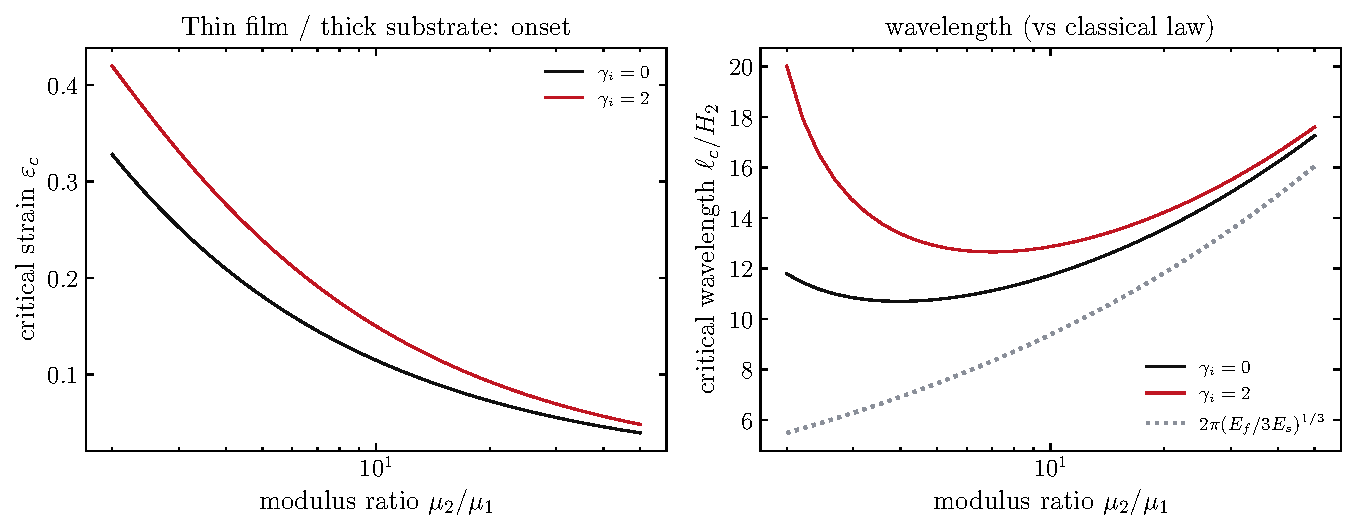
\includegraphics[width=\linewidth]{pics/bilayer_map.pdf}
	\caption{Bilayer instability with interfacial surface energy. (a)
	Critical strain $\varepsilon_c$ versus modulus ratio $\mu_2/\mu_1$
	for interfacial tension $\gamma_i=0$ (solid) and $\gamma_i>0$
	(dashed); (b) the corresponding selected wavelength
	$\ell_c/H_2$. Curves are the bilayer perturbation
	prediction~\eqref{eq:bilayer_det} for a thin film on a thick substrate
	($H_1=20,\,H_2=1$); the dotted line in (b) is the classical
	film/substrate law $2\pi(E_f/3E_s)^{1/3}$.}
	\label{fig:bilayer_map}
\end{figure}

We verify~\eqref{eq:bilayer_det} against nonlinear finite-element
calculations in which the two layers are meshed as bonded element blocks
sharing a conforming row of interface nodes, and the surface traction is
applied on both the top side set and the internal interface side set. The
laminate ($L_f=40$, substrate $H_1=8$, film $H_2=1$) is compressed
laterally under displacement control until the top-surface undulation
reaches the bifurcation, and the onset strain and wavelength are extracted
at each modulus ratio. As shown in Figure~\ref{fig:case3_fe}, the FE onset
strains track the perturbation prediction across $5\leqslant\mu_2/\mu_1
\leqslant20$, decreasing monotonically from $\varepsilon_c\approx0.18$ to
$0.08$, with the FE values lying a uniform ${\sim}10\%$ above the linear
theory---the expected offset between an infinitesimal-amplitude bifurcation
and a finite-amplitude onset measured at a small but nonzero amplitude. The
selected wavelengths likewise agree to within the discrete set permitted by
the finite specimen length. Most importantly, switching on the interfacial
tension at fixed modulus ratio ($\mu_2/\mu_1=10$) raises the onset strain
from $\varepsilon_c=0.118$ to $0.213$ in the FE calculation, in close
agreement with the corresponding shift $0.105\to0.189$ predicted
by~\eqref{eq:bilayer_det}. This confirms that interfacial surface energy is
a distinct and quantitatively accessible control parameter for the surface
morphology of layered dielectric elastomers.

\begin{figure}
	\centering
	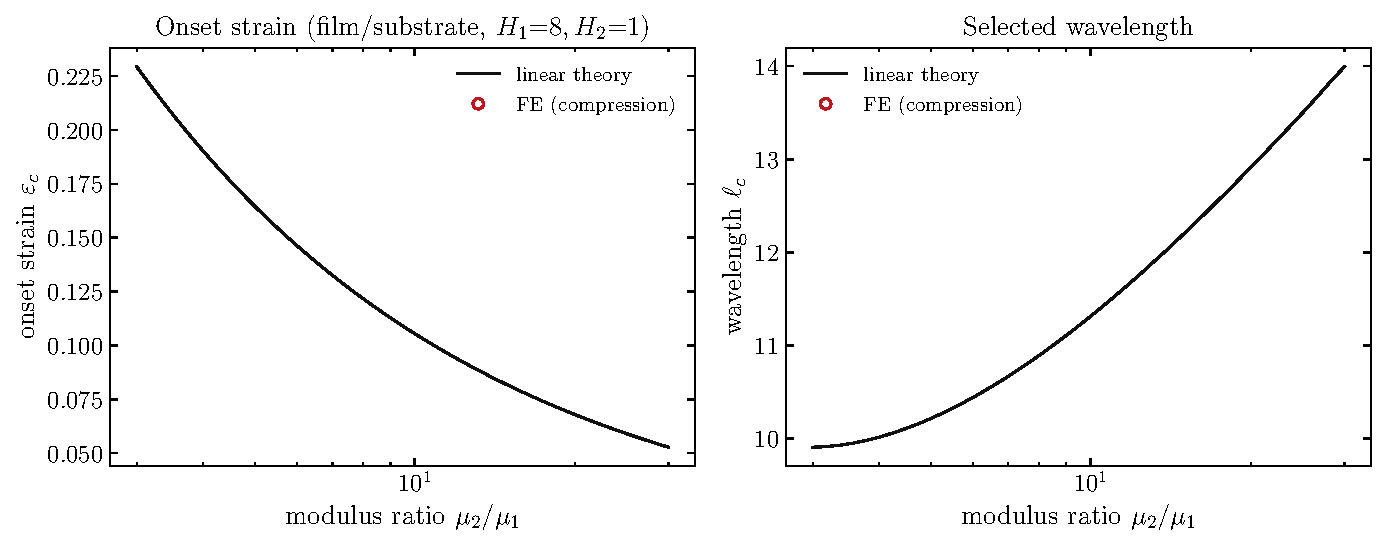
\includegraphics[width=\linewidth]{pics/case3_fe.pdf}
	\caption{Finite-element verification of the bilayer onset
	criterion~\eqref{eq:bilayer_det} for the film/substrate geometry
	($H_1=8$, $H_2=1$, $\gamma_i=0$). (a) Onset compressive strain
	$\varepsilon_c$ and (b) selected wavelength $\ell_c$ versus modulus
	ratio: solid line, linear stability theory; markers, nonlinear FE under
	lateral compression. The FE onset is measured where the top-surface
	undulation first reaches $10\%$ of the film thickness, which accounts
	for the small uniform upward offset relative to the infinitesimal-
	amplitude theory.}
	\label{fig:case3_fe}
\end{figure}

\subsection{Generalization to an $N$-layer laminate}
\label{sec:nlayer}

The bilayer construction extends directly to an arbitrary stack of $N$
bonded incompressible neo-Hookean layers, with shear moduli $\mu_k$ and
thicknesses $H_k$ ($k=1,\dots,N$, ordered from the rigid base upward) and
an independent surface tension $\gamma_i$ on each internal interface
($i=1,\dots,N-1$) in addition to the free-surface tension $\gamma_t$.
Since the bonded stack shares a single in-plane stretch $\lambda$, every
layer carries the four-mode envelope of Section~\ref{sec:multilayer} in
its own local coordinate, giving $4N$ unknown amplitudes. These are fixed
by $4N$ conditions---two at the clamped base, the four continuity/Laplace
conditions~\eqref{eq:interface_jump} at each of the $N-1$ interfaces, and
two at the free top---assembled into a banded $4N\times4N$ matrix
$\mathbf{M}(\lambda,K)$ whose vanishing determinant is the bifurcation
condition. The assembly is the standard transfer-matrix (propagator) form
and is linear in $N$, so laminates with many layers are solved at
negligible cost; the null vector of $\mathbf{M}$ at threshold yields the
mode shape, which localizes the incipient instability to a particular
surface or interface.

This generalization exposes a qualitatively new effect that the single
free surface cannot display. Consider a thin stiff sheet buried between
two soft layers. When the free-surface tension is small, compression
triggers a buckling mode of the stiff sheet that also deflects the top
surface. As $\gamma_t$ is increased, the free-surface undulation is
progressively penalized and flattened, yet the buried sheet continues to
buckle at essentially the same critical strain, because its mode is
localized away from the free surface and is therefore insensitive to
$\gamma_t$. Beyond a threshold surface tension the buried interface
buckles \emph{first}, with the top surface remaining flat
(Figure~\ref{fig:nlayer_mode}): surface tension does not merely shift the
onset of a single instability but can \emph{select which interface fails
first}, decoupling internal pattern formation from the external surface.
The same $4N\times4N$ framework provides the forward map for the inverse
design of layered actuators with a prescribed buried or surface
morphology; because each evaluation is inexpensive, it is also a natural
basis for a reduced-order surrogate over the layer parameters
$(\mu_k,H_k,\gamma_i)$ when embedded in a design-optimization loop.

\begin{figure}
	\centering
	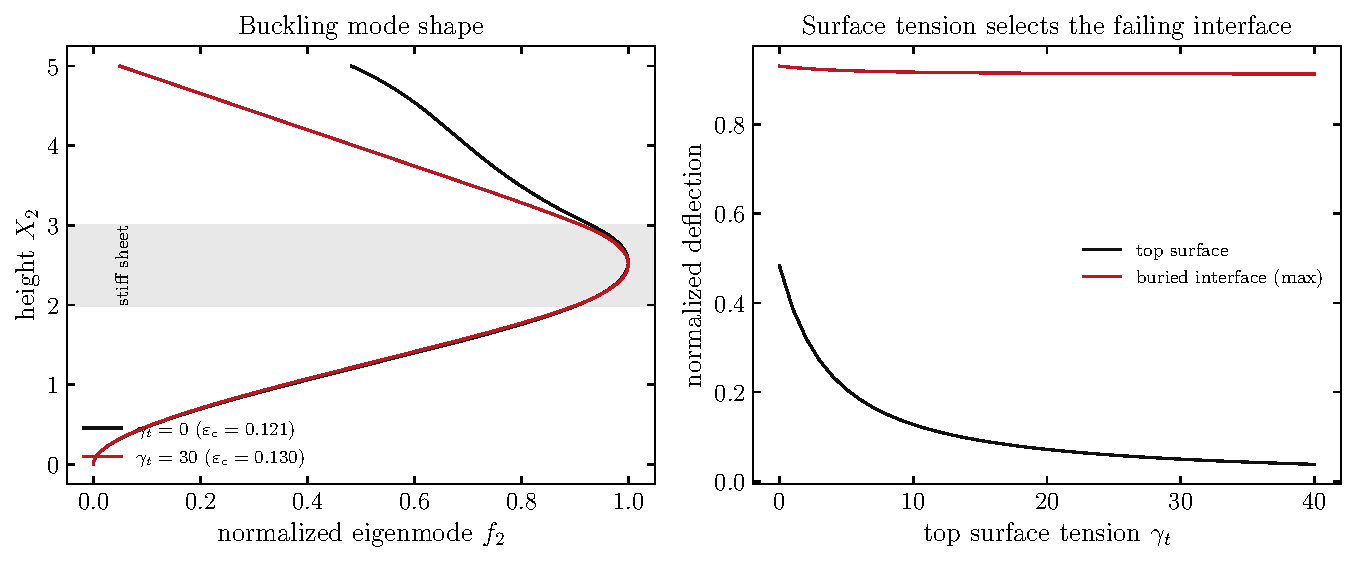
\includegraphics[width=\linewidth]{pics/nlayer_mode.pdf}
	\caption{Surface tension selects the failing interface in a
	three-layer soft/stiff/soft laminate. (a) At low free-surface
	tension the buried stiff sheet buckles and the top surface follows;
	(b) at high free-surface tension the top surface is flattened while
	the buried sheet still buckles at nearly the same critical strain, so
	the interface instability preempts the surface one. Curves are the
	normalized vertical-displacement eigenmode $f_2(X_2)$ from the
	$N$-layer determinant.}
	\label{fig:nlayer_mode}
\end{figure}

\section{Conclusions}

We have extended the elastocapillary wrinkling analysis of compressed dielectric elastomers from a single film to multilayer laminates, and verified it with nonlinear finite-element calculations. Surface energy on a buried interface between dissimilar dielectric layers enters the bifurcation problem as a Laplace-pressure jump in the normal traction~\eqref{eq:interface_jump}, raising the critical strain and coarsening the selected wavelength much as free-surface tension does; the bilayer determinant reduces correctly to the homogeneous Biot limit and to the classical stiff-film/soft-substrate wrinkling law. For laminates of three or more layers a qualitatively new effect emerges: a sufficiently large free-surface tension flattens the outer surface while a buried stiff layer continues to buckle, so that surface tension selects which interface fails first. On the computational side, the same edge-based Young--Laplace surface stress is applied on internal interfaces exactly as on free surfaces, by declaring the interface as an element side set. Interfacial energy thus emerges as an additional, independently tunable control over the surface morphology of layered soft actuators, and the $N$-layer determinant provides a compact forward model for their design.

\appendix
\section{Finite-element application of surface tension on an internal interface}
\label{app:interface}

The free-surface Young--Laplace traction used here was introduced and validated for the \emph{exterior} surface of a single body in~\citet{seifiIJSS2016}. The multilayer results of Section~\ref{sec:multilayer} require the same surface energy on a buried \emph{interface} between two bonded layers. We summarize how this is done without altering the surface constitutive model; only the set of faces on which it acts is extended.

\paragraph{Discrete surface stress.} The surface energy is carried on the element edges that lie on the surface. For a deformed surface edge with end nodes at current positions $\mathbf{x}_a,\mathbf{x}_b$, let $\Delta\mathbf{x}=\mathbf{x}_a-\mathbf{x}_b$ with current length $\ell=|\Delta\mathbf{x}|$. The edge carries the constant Young--Laplace surface stress $\sigma_s=\gamma$, with $\gamma$ the surface tension. The corresponding nodal forces are
\begin{equation}
	\mathbf{f}_a=-\frac{\sigma_s}{\ell}\,\Delta\mathbf{x},\qquad
	\mathbf{f}_b=+\frac{\sigma_s}{\ell}\,\Delta\mathbf{x},
\end{equation}
so each edge pulls its end nodes together along the deformed tangent with magnitude $\sigma_s$. At a node shared by two surface edges the net force is $\sigma_s(\hat{\mathbf{t}}_2-\hat{\mathbf{t}}_1)$, proportional to the discrete curvature times the tension---the discrete Laplace pressure---and the consistent geometric and material tangent contributions are assembled likewise.

\paragraph{Extension to an interface.} On a free surface the active faces are the exterior element faces, identified automatically as those without a neighboring element. An internal interface between two element blocks is fully surrounded by material and is therefore \emph{not} detected as a free surface. To apply surface energy there, the interface is declared as an element side set and supplied to the surface-tension input exactly as a free surface would be. The element then (i)~collects the side-set faces, (ii)~merges their parent elements into the surface-element list---these are otherwise absent, having no exterior face---and (iii)~marks the designated faces as active. The identical edge-based stress $\sigma_s$ and nodal forces are then evaluated on the interface edges. Because the two layers are meshed conformally and share the interface nodes (a bonded, displacement-continuous interface), the curvature-driven force acts on the shared nodes and is transmitted to both layers, realizing the interfacial Laplace-pressure jump of Eq.~\eqref{eq:interface_jump}.

Two consequences follow. First, because the surface constitutive model is unchanged and only the face set is extended, the prior validation of the free-surface model carries over to the interface. Second, surface tensions are specified per side set, so distinct values may be assigned to the top surface and to each internal interface independently, as exploited in Section~\ref{sec:nlayer}.

\section{Acknowledgements}

HSP and SS acknowledge funding from the ARO, grant W911NF-14-1-0022.

\bibliography{biball,park_holmes_nsf_2016}

\end{document}